\section{Array performance} \label{sec:beamforming_array_spl}

The aim of this section is to evaluate the frequency reponse performance of the beamforming array. It has been shown in \autoref{sec:main_axis}, that the sound pressure in front of the beamforming array does not act linear from \SI{60}{\hertz} to \SI{300}{\hertz} and for that reason a cost filter has been introduced. This section will evaluate the effects of implementing the cost filter for the \gls{sp}-parameters used in the measurement (\autoref{ax:directional_3}). The measured polar respone of a the speaker array without \gls{sp} applied is used as reference. 
The measured reference case does not match the setup used for reference in the analytical considerations in \autoref{sec:main_axis}, where all of the speakers are placed on a line (\autoref{fig:ref_omni_array}). It has not been possible to recreate the setup with reasonable effort because of physical constrains. Another speaker mounting contraption would be necessary and size of the cabinets makes it impossible to place the acoustic centers according to the specification without tilting the azimuth of the outside speakers. Since the acoustic center of speaker B and C in \autoref{fig:ref_omni_array} have to be \SI{40}{\centi\meter} apart, and theys cabinet both are \SI{40}{\centi\meter} in width, the most simple way to place them is against each other. This leaves no space for speaker A.
It has therefore been decided to stick to the speaker positions of the array that are used during beamforming.
% Therefore it has been decided that the comparing between beamforming array and omnidirectional array is done with the same position but when the array in in omnidirectional mode all speaker gets the same signal. It would have been possible to build a new stand, where speaker A was placed such that at  least all the acoustical center was aligned with the right distance. This stand was not build.

The measurements that are compared are described in \autoref{sec:05_11_results}, where the beamforming is enabled and disabled. The reference sweep (\autoref{fig:time_signal}) is played back through all of speakers as a test signal, when the beamforming is disabled. Therefore comparing the pressure with the one measured with beamforming enabled is possible. Ideally, the difference of those two measurements would be zero if the cost filter is working prefectly, the acoustic centers of the speakers are positioned exactly and there is no influence of the speakes cabinets on the sound field. The following \autoref{fig:beamforming_off_on} shows the \gls{spl} in front of the array on the main axis with and without beamforming.

  \begin{figure}[H]
	\centering
	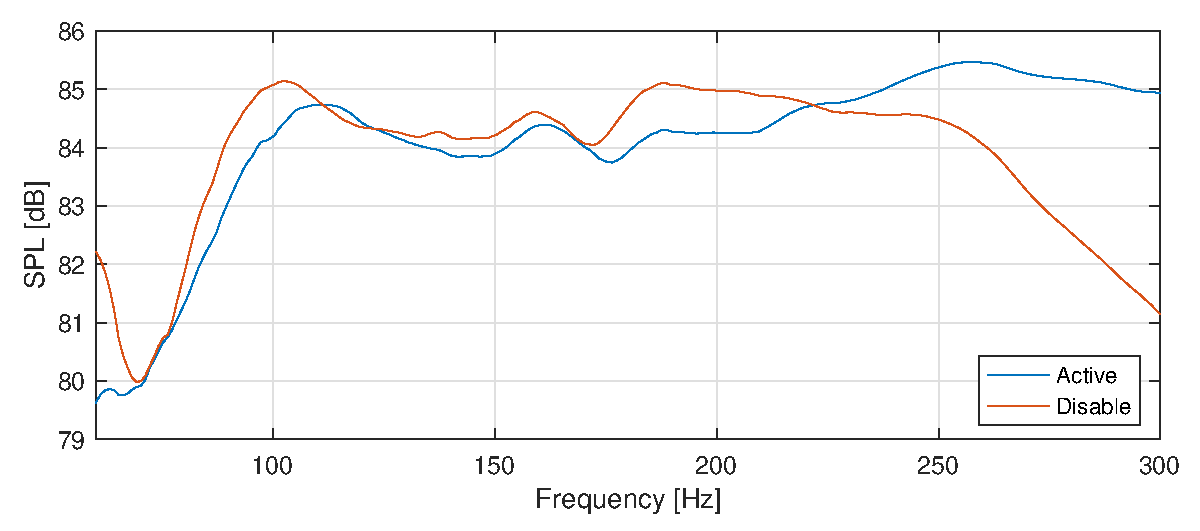
\includegraphics[width=1\textwidth]{beamforming_off_on.eps}
	\caption{The figure shows the \gls{spl} in front for the array at a distance of \SI{4.92}{\meter}, where the blue graph is with beamforming enabled and the red graph is without beamforming.}
		\label{fig:beamforming_off_on}
\end{figure}


In \autoref{fig:beamforming_off_on} the graph with and without beamforming shows that the cost filter is functional and actually works very well from \SI{70}{\hertz} to \SI{250}{\hertz}. Outside that frequency range, the graph shows, that frequency response of the array with beamforming diverges from that of configuration without beamforming. As explained, the cost filter has been designed with aligned aligned speakers as reference, whereas both measurements have been conducted with the triangular setup. This is likely to have an influence. To investigate the difference between the aligned setup and the triangle setup with disabled beamforming, the difference between the two will be calculated analytically. The following \autoref{fig:beamforming_aligned_triangle} shows the relative pressure of both analytical models with the aligned model as reference.

  \begin{figure}[H]
	\centering
	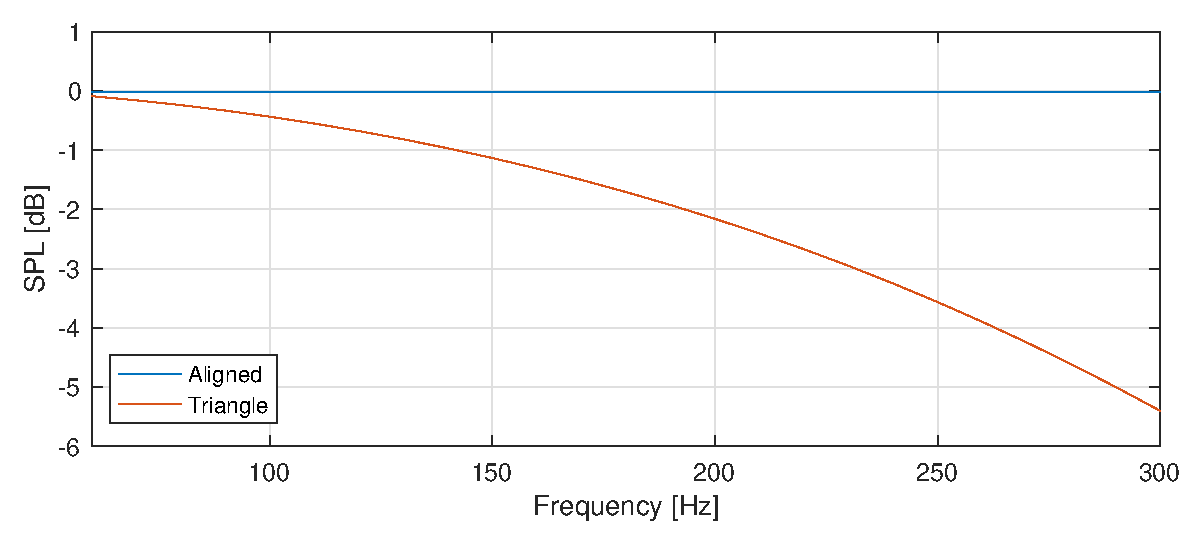
\includegraphics[width=1\textwidth]{beamforming_aligned_triangle.eps}
	\caption{Relative pressure in front for the aligned array and the triangular array without beamforming}
		\label{fig:beamforming_aligned_triangle}
\end{figure}

The difference in the analytical models in \autoref{fig:beamforming_aligned_triangle} shows that the pressure between the aligned setup and the triangular setup without beamforming is different. The triangular setup drops in pressure when the frequency rises towards \SI{300}{\hertz} like in \autoref{fig:beamforming_off_on} but more drastic. This shows, that changing the reference for beamforming cost from an aligned setup to the triangular setup leads to a change in cost especially in the high frequency, just as seen in \autoref{fig:beamforming_off_on}. This change of reference is likely to be one of the reasons leading to the graph with beamforming disabled in \autoref{fig:beamforming_off_on} diverging towards higher frequencies. The following \autoref{fig:beamforming_off_on_corrected} shows the graph where the calculated difference from \autoref{fig:beamforming_aligned_triangle} is added to the measured frequency response of the triangle without beamforming in  \autoref{fig:beamforming_off_on}.

  \begin{figure}[H]
	\centering
	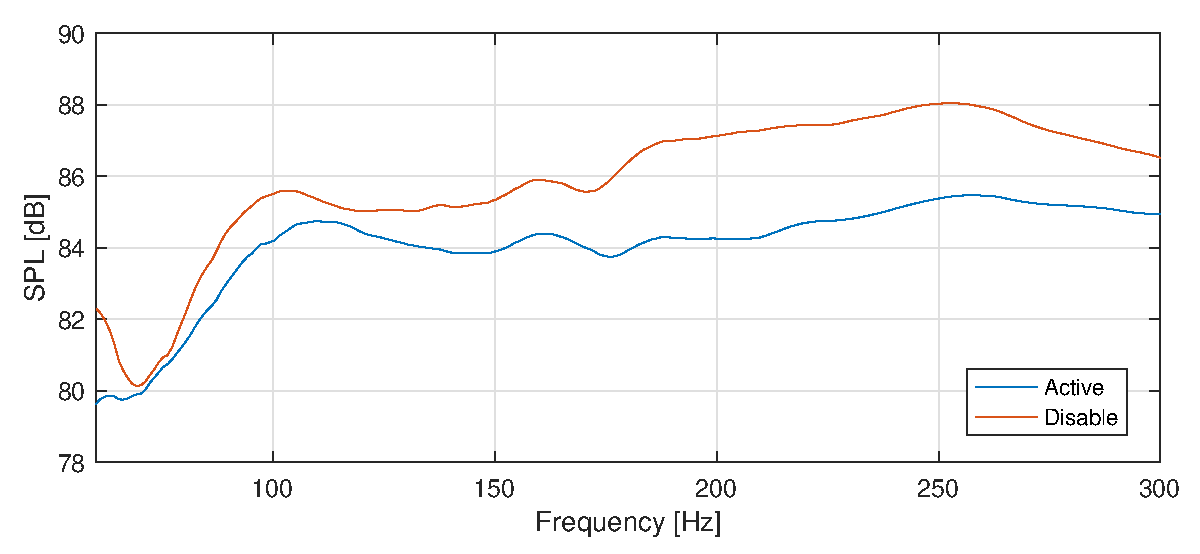
\includegraphics[width=1\textwidth]{beamforming_off_on_corrected.eps}
	\caption{The figure shows the \gls{spl} in front for the array with a distance of \SI{4.92}{\meter}, where the blue graph is with beamforming and the red graph is without beamforming and with the analytical correction}
		\label{fig:beamforming_off_on_corrected}
\end{figure}

At this point, the cost filter seems to fit very well according to the graphs in \autoref{fig:beamforming_off_on_corrected}. It can be seen that there is a gain offset of approx. \SI{2}{\decibel}, in terms of shape, both graphs are very similar. 

To investigate, how the beamforming filter affects the sound pressure all around the speaker array. Therefore the difference in sound pressure level between enabled and disabled beamforming will presented next. The formerly mentioned analytical correction is not incorporated in the polar plot. The following \autoref{fig:polar_plot_dif_result} shows the polar plot of the pressure difference. 


 \begin{figure}[H]
	\centering
	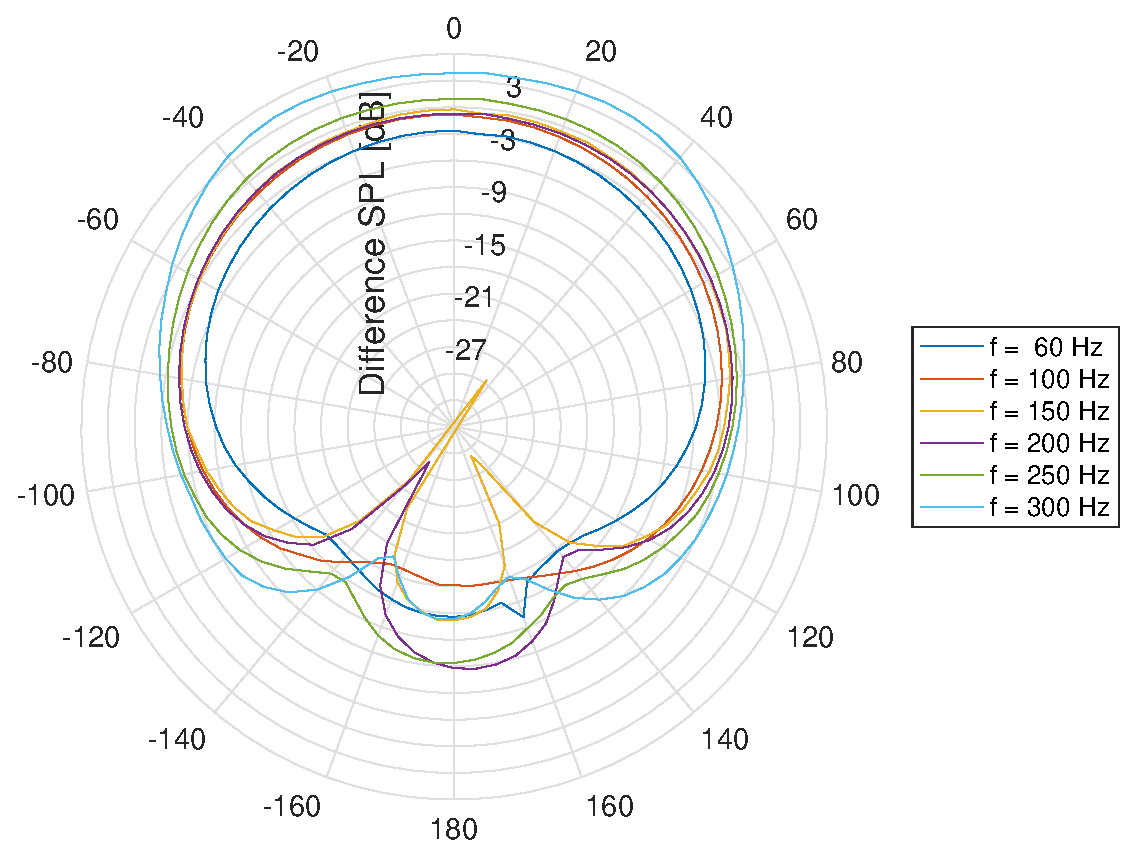
\includegraphics[width=0.9\textwidth]{polar_plot_dif_result.eps}
	\caption{Polar plot of the \gls{spl} difference around the array with enabled and disabled beamforming.}
		\label{fig:polar_plot_dif_result}
\end{figure}




\section{Conclusion}
In order to make a meaningful comparison between the measurements, an analytical correction accounting for the change in reference setup has to be applied. When this is done, it can be concluded that the cost filter works as intended, apart from an approx. \SI{2}{\decibel} gain difference measured over most of the frequency range.


